\section{HÌNH BÌNH HÀNH - HÌNH THOI}
\subsection{Hình bình hành}
\subsubsection{Kiến thức trọng tâm}

\begin{dn}
\immini{
Hình bình hành là tứ giác có các cạnh đối song song.
}
{
\begin{tikzpicture}[line join=round, line cap = round, >=stealth, scale=1,font=\footnotesize,transform shape]
\def \g{60}
\path 
(0,0) coordinate (A)
({\g}:1.5) coordinate (B)
(3,0) coordinate (D)
($(B)+(D)-(A)$) coordinate (C) 
;
\draw (A)--(B)--(C)--(D)--(A);
\foreach \x/\g in {A/-140,B/120,C/50,D/-40}
\fill[black] (\x) circle(1pt) +  (\g:3mm) node {$\x$};
\end{tikzpicture}
}
\end{dn}

\begin{dl}
Trong hình bình hành:
\immini{
\begin{itemize}
\item Các cạnh đối bằng nhau.
\item Các góc đối bằng nhau.
\item Hai đường chéo cắt nhau tại trung điểm của mỗi đường.
\end{itemize}
}
{
\begin{tikzpicture}[line join=round, line cap = round, >=stealth, scale=1,font=\footnotesize,transform shape]
\def \g{60}
\path 
(0,0) coordinate (A)
({\g}:1.8) coordinate (B)
(4,0) coordinate (D)
($(B)+(D)-(A)$) coordinate (C) 
($(A)!0.5!(C)$) coordinate (O) 
;
\draw (A)--(B)--(C)--(D)--(A) (A)--(C)  (B)--(D);
\draw pic[draw=black,double, angle eccentricity=0.66, angle radius=0.5cm] {angle=D--A--B};
\draw pic[draw=black,double, angle eccentricity=0.66, angle radius=0.6cm] {angle=B--C--D};
\draw pic[draw=black, angle eccentricity=0.66, angle radius=0.4cm] {angle=A--B--C};
\draw pic[draw=black, angle eccentricity=0.66, angle radius=0.3cm] {angle=C--D--A};
\draw (A)--(B)node[midway,rotate=60]{$|$};
\draw (C)--(B)node[midway]{$||$};
\draw (C)--(D)node[midway,rotate=60]{$|$};
\draw (A)--(D)node[midway]{$||$};
\foreach \x/\g in {A/-140,B/120,C/50,D/-40,O/90}
\fill[black] (\x) circle(1pt) +  (\g:3mm) node {$\x$};
\end{tikzpicture}
}
\end{dl}

\begin{luuy}
\textbf{Dấu hiệu nhận biết} \\
Ta có các dấu hiệu nhận biết một tứ giác là hình bình hành như sau:
\begin{enumerate}
\item  Tứ giác có các cạnh đối song song là hình bình hành.
\item  Tứ giác có các cạnh đối bằng nhau là hình bình hành.
\item  Tứ giác có hai cạnh đối song song và bằng nhau là hình bình hành.
\item  Tứ giác có các góc đối bằng nhau là hình bình hành.
\item  Tứ giác có hai đường chéo cắt nhau tại trung điểm của mỗi đường là hình bình hành.
\end{enumerate}
\end{luuy}

\subsubsection{Các ví dụ}
\begin{vd}%[Đề Cương Toán 8]%[Phạm Tuấn]%[8H5H4-4]
Hình bình hành $ABCD$ có $\widehat{A}=35^{\circ}$. Tính số đo các góc còn lại của hình bình hành đó.
\loigiai{
\immini{
$ABCD$ là hình bình hành nên $\widehat{A} = \widehat{C} =35^\circ$. \\
Ta lại có $AD \parallel BC$ nên $\widehat{A} + \widehat{B} = 180^\circ$, suy ra $\widehat{B}= \widehat{D} = 135^\circ$.
}
{
\begin{tikzpicture}[line join=round, line cap = round, >=stealth, scale=1,font=\footnotesize,transform shape]
\def \g{35}
\path 
(0,0) coordinate (A)
({\g}:1.5) coordinate (B)
(3,0) coordinate (D)
($(B)+(D)-(A)$) coordinate (C) 
;
\draw (A)--(B)--(C)--(D)--(A);
\foreach \x/\g in {A/-140,B/120,C/50,D/-40}
\fill[black] (\x) circle(1pt) +  (\g:3mm) node {$\x$};
\end{tikzpicture}
}
}
\end{vd}




\begin{vd}%[Đề Cương Toán 8]%[Phạm Tuấn]%[8H5H4-3]
Cho  hình bình hành $MNOP$ có $MO$ và $NP$ cắt nhau tại $I$ và $IN=3$ cm, $IO=4$ cm, $ON=6$ cm. Tìm độ dài cạnh $MP$ và hai đường chéo $MO$, $NP$.
\loigiai{
\immini{
Tứ giác $MNOP$ là hình bình hành nên $MP= ON=6$ cm, $MO=2OI=8$ cm, $NP=2IN=6$ cm.
}
{
\begin{tikzpicture}[line join=round, line cap = round, >=stealth, scale=0.8]
\def \g{-15}
\path 
(0,0) coordinate (M)
(0,-3) coordinate (N)
({\g}:4.5) coordinate (P)
($(N)+(P)-(M)$) coordinate (O) 
($(M)!0.5!(O)$) coordinate (I) 
;
\draw (M)--(N)--(O)--(P)--(M) (M)--(O) (N)--(P);
\foreach \x/\g in {M/120,N/-120,O/-90,P/80,I/90}
\fill[black] (\x) circle(1pt) +  (\g:3.5mm) node {$\x$};
\end{tikzpicture}
}
}
\end{vd}

\begin{vd}%[Đề Cương Toán 8]%[Phạm Tuấn]%%[8H5H4-2]
Cho tứ giác $ABCD$ có $\widehat{A}= \widehat{C}= 40^\circ$, $\widehat{B}=140^\circ$. Chứng minh tứ giác $ABCD$ là hình bình hành.
\loigiai{
Ta có $\widehat{A}+ \widehat{B}+ \widehat{C}+ \widehat{D} = 360^\circ$, do đó $\widehat{D}= 360^\circ- 80^\circ -140^\circ = 140^\circ$. \\
Tứ giác $ABCD$ có các góc đối bằng nhau nên là hình bình hành.
}
\end{vd}

\begin{vd}%[Đề Cương Toán 8]%[Phạm Tuấn]%[8H5H4-2]
Cho hình bình hành $ABCD$ có $M$, $N$ lần lượt là trung điểm các cạnh $AB$ và $CD$. Chứng minh rằng tứ giác $AMCN$ là hình bình hành.
\loigiai{
\immini{
Tứ giác $ABCD$ là hình bình hành nên $AB=CD$ và $AB=CD$. \\
Theo giả thiết $M$, $N$ lần lượt là trung điểm các cạnh $AB$ và $CD$ suy ra $AM=\dfrac{1}{2}AB = \dfrac{1}{2}CD=  CN$. \\
Mặt khác $AM \parallel CN$, do đó tứ giác $AMCN$ là hình bình hành.
}
{
\begin{tikzpicture}[line join=round, line cap = round, >=stealth, scale=1]
\def \g{60}
\path 
(0,0) coordinate (A)
({\g}:2) coordinate (B)
(3.5,0) coordinate (D)
($(B)+(D)-(A)$) coordinate (C) 
($(A)!0.5!(B)$) coordinate (M) 
($(C)!0.5!(D)$) coordinate (N) 
;
\draw (A)--(B)--(C)--(D)--(A) (M)--(C) (A)--(N);
\foreach \x/\g in {A/-140,B/120,C/50,D/-40,M/170,N/-10}
\fill[black] (\x) circle(1pt) +  (\g:3mm) node {$\x$};
\end{tikzpicture}
}
}
\end{vd}

\begin{vd}%[Đề Cương Toán 8]%[Phạm Tuấn]%[8H5H4-2]
Cho hình bình hành $ABCD$ tâm $O$. Trên cạnh $OA$ lấy điểm $M$ sao cho $AM= \dfrac{2}{3} AO$, trên cạnh $OC$ lấy điểm $N$ sao cho $CN= \dfrac{2}{3} CO$. Tứ giác $BMDN$ là hình gì? Tại sao?
\loigiai{
\immini{
Tứ giác $ABCD$ là hình bình hành nên $OA=OC$, $OB=OD$.  \\
Mà theo giả thiết $AM= \dfrac{2}{3} AO$ và $CN= \dfrac{2}{3} CO$, suy ra $OM=ON$. \\
Khi đó, tứ giác $BMDN$ có hai đường chéo cắt nhau tại trung điểm mỗi đường nên là hình bình hành.
}
{
\begin{tikzpicture}[line join=round, line cap = round, >=stealth, scale=1]
\def \g{60}
\path 
(0,0) coordinate (A)
({\g}:2.5) coordinate (B)
(4.5,0) coordinate (D)
($(B)+(D)-(A)$) coordinate (C) 
($(A)!0.5!(C)$) coordinate (O)
($(A)!0.66!(O)$) coordinate (M) 
($(C)!0.66!(O)$) coordinate (N) 
;
\draw (C)--(A)--(B)--(C)--(D)--(A) (B)--(M)--(D)--(N)--(B)--(D);
\foreach \x/\g in {A/-140,B/120,C/50,D/-40,M/170,N/-10,O/90}
\fill[black] (\x) circle(1pt) +  (\g:4mm) node {$\x$};
\end{tikzpicture}
}
}
\end{vd}

\begin{vd}%[Đề Cương Toán 8]%[Phạm Tuấn]%[8H5H4-2]
Cho hai hình bình hành $ABCD$. Trên tia đối tia $CB$ lấy điểm $F$, trên tia đối tia $DA$ lấy điểm $E$ sao cho $EF \parallel CD$. Tứ giác $ABFE$ là hình gì? Tại sao?
\loigiai{
\immini{
Tứ giác $ABCD$ là hình bình hành nên $AB\parallel CD$ và $AD \parallel BC$. \\
Mà $CD \parallel EF$, suy ra $AB \parallel EF$. \\
Tứ giác $ABFE$ có các cặp cạnh đối song song nên là hình bình hành.
}
{
\begin{tikzpicture}[line join=round, line cap = round, >=stealth, scale=1]
\def \g{60}
\path 
(0,0) coordinate (A)
({\g}:2) coordinate (B)
(3.5,0) coordinate (D)
(5,0) coordinate (E)
($(B)+(D)-(A)$) coordinate (C) 
($(C)+(E)-(D)$) coordinate (F)
;
\draw (A)--(B)--(C)--(D)--(A) (C)--(F)--(E)--(D);
\foreach \x/\g in {A/-140,B/120,C/50,D/-90,E/-40,F/40}
\fill[black] (\x) circle(1pt) +  (\g:3mm) node {$\x$};
\end{tikzpicture}
}
}
\end{vd}
\subsubsection{Bài tập vận dụng}

\begin{bt}%[Đề Cương Toán 8]%[Phạm Tuấn]%[8H5H4-2]
Cần thêm một điều kiện gì để mỗi tứ giác trong các hình sau trở thành hình bình hành?
	\begin{multicols}{2}
		\begin{enumerate}
			
			\item \begin{tikzpicture}[line join = round, line cap = round,>=stealth,font=\footnotesize,scale=1]
				\draw	(0,0)coordinate(E)--++(-35:4)coordinate(H) node[midway]{||}--++(10:2)coordinate(G)--node[midway]{||}(10:2)coordinate(F)--cycle;
				\foreach \x/\g in {F/45,G/-45,H/-135,E/135}
				{\draw [fill=black](\x) circle (1.2pt) +(\g:3mm)node{$\x$};}
			\end{tikzpicture}
			\item 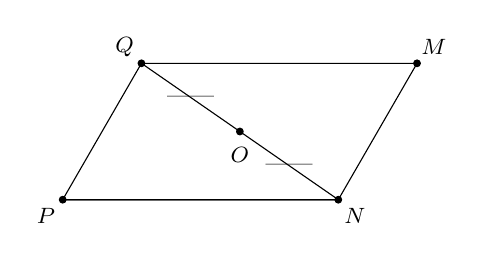
\begin{tikzpicture}[line join = round, line cap = round,>=stealth,font=\footnotesize,scale=1]
				\draw	(0,0)coordinate(P)--(3.5,0)coordinate(N)--++(60:2)coordinate(M)--(60:2)coordinate(Q)--cycle;
				\path (intersection of Q--N and M--P) coordinate (O)	% Giao điểm của hai đường thẳng
				;
				\draw (Q)--(O)node[midway]{||}--(N)node[midway]{||} (N)--(P);
				\foreach \x/\g in {Q/135,M/45,N/-45,P/-135,O/-90}
				{\draw [fill=black](\x) circle (1.2pt) +(\g:3mm)node{$\x$};}
			\end{tikzpicture}
			
		\end{enumerate}
	\end{multicols}
\loigiai{
\begin{enumerate}
\item Tứ giác $EFGH$ là hình bình hành khi có thêm điều kiện $EF=GH$ hoặc $EH \parallel FG$.
\item  Tứ giác $MNPQ$ là hình bình hành khi có thêm điều kiện $O$ là trung điểm của đoạn thẳng $MP$.
\end{enumerate}
}
\end{bt}


\begin{bt}%[Đề Cương Toán 8]%[Phạm Tuấn]%[8H5H4-5]
\immini{
Bàn vẽ có hai chân bàn $AB$ và $CD$ được gắn với nhau theo hình chữ $X$ tại trung điểm $O$ của chân $AB$. Điểm $O$ có thể di chuyển dọc theo chân bàn $CD$ để điều chỉnh độ nghiêng của mặt bàn. Điểm $O$ ở vị trí nào trên đoạn thẳng $CD$ thì cạnh bàn $BC$ song song với đường thẳng $AD$ trên mặt đất? Khi đó $ACBD$ là hình gì?
}
{
\begin{tikzpicture}[line join=round, line cap = round, >=stealth, scale=0.4,font=\footnotesize]
\path 
(0,0) coordinate (A)
(0.81,0) coordinate (A')
(6.28,11.32) coordinate (B)
($(A')+(B)-(A)$) coordinate (B')
(0.25,8.83) coordinate (C)
(7.86,0) coordinate (D)
(8.75,0) coordinate (D')
($(C)+(D')-(D)$) coordinate (C')
($(A)!0.5!(A')$) coordinate (A1)
($(D)!0.5!(D')$) coordinate (D1)
(-3.15,7.6) coordinate (E)
(10.5,13.25) coordinate (E')
(-2.86,7.01) coordinate (F)
($(F)+(E')-(E)$) coordinate (F')
(intersection of A--B and F--F') coordinate (X)
(intersection of A'--B' and F--F') coordinate (X')
(intersection of C--D and F--F') coordinate (Y)
(intersection of C'--D' and F--F') coordinate (Y')
($(X)!0.5!(X')$) coordinate (B1)
($(Y)!0.5!(Y')$) coordinate (C1)
(intersection of A1--B1 and C1--D1) coordinate (O)
($(C1)!0.5!(O)$) coordinate (O1)
($(O1)!2!(O)$) coordinate (O2)
($(O)!2!(O2)$) coordinate (O3)
($(O2)!2!(O3)$) coordinate (O4)
;
\draw[fill=brown!80!black] (A)--(A')--(B')--(B)--(A) ;
\draw[fill=brown!80!black] (C)--(C')--(D')--(D)--(C) ;
\draw[fill=brown!80!black] (E)--(E')--(F')--(F)--(E) ;
\draw[thick] (-2.5,0)--(12.5,0) ;
\foreach \x/\g in {O/-120,O1/90,O2/10,O3/10,O4/10}
\fill[black] (\x) circle(5pt) +  (\g:3mm) node {};
\draw[fill] (A1) circle(2pt) node[below]{$A$} (B1)circle(2pt)  node[below right]{$B$} (C1) circle(2pt) node[below left]{$C$} (D1) circle(2pt) node[below]{$D$}; 
\end{tikzpicture}
}
\loigiai{
Khi $AD \parallel BC$, ta có $\widehat{OAD} = \widehat{OBC}$ (so le trong). \\
Xét tam giác $OAD$ và $OBC$ có $\heva{&\widehat{OAD} = \widehat{OBC}\\&OA=OB\\&\widehat{AOD} = \widehat{BOC}.}$ \\
Suy ra hai tam giác $OAD$ và $OBC$  bằng nhau, do đó $OC=OD$.  \\
Khi đó tứ giác $ACBD$ có hai đường chéo cắt nhau tại trung điểm mỗi đường nên là hình bình hành.
}
\end{bt}

\begin{bt}%[Đề Cương Toán 8]%[Phạm Tuấn]%[8H5H4-2]
Cho hình bình hành $ABCD$ tâm $O$. Kẻ $BM$, $DN$ cùng vuông góc với $AC$.  Tứ giác $BMDN$ là hình gì? Tại sao?
\loigiai{
\immini{
Tứ giác $ABCD$ là hình bình hành nên $OA=OC$, $OB=OD$.  \\
Hai tam giác $BMO$ và $DNO$ có $\heva{&OB=OD\\&\widehat{BOM} = \widehat{DON}\\& \widehat{M}= \widehat{N}=90^\circ }$, suy ra $\triangle BMO = \triangle DNO$. Do đó $OM=ON$. \\
Tứ giác $BMDN$ có hai đường chéo cắt nhau tại trung điểm mỗi đường nên là hình bình hành.
Khi đó, tứ giác $BMDN$ có hai đường chéo cắt nhau tại trung điểm mỗi đường nên là hình bình hành.
}
{
\begin{tikzpicture}[line join=round, line cap = round, >=stealth, scale=1]
\def \g{60}
\path 
(0,0) coordinate (A)
({\g}:2.5) coordinate (B)
(4.5,0) coordinate (D)
($(B)+(D)-(A)$) coordinate (C) 
($(A)!0.5!(C)$) coordinate (O)
($(A)!(B)!(C)$) coordinate (M) 
($(A)!(D)!(C)$) coordinate (N) 
;
\draw (C)--(A)--(B)--(C)--(D)--(A) (B)--(M)--(D)--(N)--(B)--(D);
\foreach \x/\g in {A/-140,B/120,C/50,D/-40,M/170,N/-10,O/90}
\fill[black] (\x) circle(1pt) +  (\g:4mm) node {$\x$};
\end{tikzpicture}
}
}
\end{bt}

\begin{bt}%[Đề Cương Toán 8]%[Phạm Tuấn]%[8H5H4-2]
\immini{
Cho hai hình bình hành $ABCD$ và $ABEF$ có chung cạnh $AB$. Chứng minh rằng tứ giác $CDFE$ là hình bình hành.
}
{
\begin{tikzpicture}[line join=round, line cap = round, >=stealth, scale=1,font=\footnotesize,transform shape]
\def \g{120}
\path 
(0,0) coordinate (A)
(3,0) coordinate (B)
({-\g}:1.5) coordinate (D)
($(B)+(D)-(A)$) coordinate (C) 
(110:1.5) coordinate (F)
($(B)+(F)-(A)$) coordinate (E) 
;
\draw (A)--(B)--(C)--(D)--(A) (A)--(F)--(E)--(B)  (C)--(E)  (D)--(F);
\foreach \x/\g in {A/160,B/0,C/-40,D/-140,E/60,F/120}
\fill[black] (\x) circle(1pt) +  (\g:3mm) node {$\x$};
\end{tikzpicture}
}
\loigiai{
$ABCD$ là hình bình hành nên $AB = CD$ và $AB \parallel CD$. \\
$ABEF$ là hình bình hành nên $AB = EF$ và $AB \parallel EF$.  \\
Suy ra  $CD=EF$ và $CD \parallel EF$ suy ra tứ giác $ABCD$ là hình bình hành.
}
\end{bt}

%%%%%%%%%%%%%%%%

\begin{bt}%[Đề Cương Toán 8]%[Phạm Tuấn]%[8H5H4-2]
Cho hình bình hành $ABCD$ có $M$, $N$, $E$, $F$ lần lượt là trung điểm các cạnh $AB$, $CD$, $BC$, $AD$. Đường thẳng $BF$ cắt các đường thẳng $CM$, $AN$ lần lượt tại $P,Q$, Đường thẳng $DE$ cắt các đường thẳng $AN$, $CM$ lần lượt tại $R,Q$. Chứng minh rằng tứ giác $PQRS$ là hình bình hành.
\loigiai{
\immini{
Tứ giác $ABCD$ là hình bình hành nên $AB=CD$ và $AB=CD$. \\
Theo giả thiết $M$, $N$ lần lượt là trung điểm các cạnh $AB$ và $CD$ suy ra $AM= CN$ và $AM \parallel CN$. \\
Do đó tứ giác $AMCN$ là hình bình hành, suy ra $AN \parallel CM$ hay $PS \parallel QR$. \\
Chứng minh tương tự ta được $BFDE$ là hình bình hành, suy ra $BF\parallel DE$ hay $PQ \parallel RS$. \\
Tứ giác $PQRS$ có các cặp cạnh đối song song nên là hình bình hành.
}
{
\begin{tikzpicture}[line join=round, line cap = round, >=stealth, scale=1]
\def \g{60}
\path 
(0,0) coordinate (A)
({\g}:3) coordinate (B)
(4,0) coordinate (D)
($(B)+(D)-(A)$) coordinate (C) 
($(A)!0.5!(B)$) coordinate (M) 
($(C)!0.5!(D)$) coordinate (N) 
($(B)!0.5!(C)$) coordinate (E) 
($(A)!0.5!(D)$) coordinate (F) 
($(M)!0.2!(C)$) coordinate (P) 
($(M)!0.6!(C)$) coordinate (S) 
($(A)!0.4!(N)$) coordinate (Q) 
($(A)!0.8!(N)$) coordinate (R) 
;
\draw (A)--(B)--(C)--(D)--(A) (M)--(C) (A)--(N) (B)--(F)  (D)--(E);
\foreach \x/\g in {A/-140,B/120,C/50,D/-40,M/170,N/-10,E/90,F/-90,P/160,Q/150,R/-130,S/-40}
\fill[black] (\x) circle(1pt) +  (\g:3mm) node {$\x$};
\end{tikzpicture}
}
}
\end{bt}




%%%%%%%%%%%%%%%

\begin{bt}%[Đề Cương Toán 8]%[Phạm Tuấn]%[8H5H4-2]
Cho tam giác $ABC$ có $O$ là trung điểm của $AC$. Trên tia đối của tia $OB$ lấy điểm $D$ sao cho $O$ là trung điểm của $BD$.
	\begin{enumerate}
		\item Chứng minh tứ giác $ABCD$ là hình bình hành.
		\item Trên tia đối của tia $CD$ lấy điểm $E$ sao cho $C$ là trung điểm của $DE$. Chứng minh $BE \parallel AC$.
	\end{enumerate}
	\loigiai
	{
		\begin{center}
			\begin{tikzpicture}[line join=round, line cap = round, >=stealth, scale=1]
\def \g{60}
\path 
(0,0) coordinate (A)
({\g}:2.5) coordinate (B)
(4.5,0) coordinate (D)
($(B)+(D)-(A)$) coordinate (C) 
($(A)!0.5!(C)$) coordinate (O)
($(C)!-1!(D)$) coordinate (E) 
;
\draw (C)--(A)--(B)--(C)--(D)--(A) (B)--(D) (A)--(C) (B)--(E)--(C);
\foreach \x/\g in {A/-140,B/120,C/10,D/-40,E/90,O/90}
\fill[black] (\x) circle(1pt) +  (\g:4mm) node {$\x$};
\end{tikzpicture}
		\end{center}
		\begin{enumerate}
			\item Do tứ giác $ABCD$ có hai đường chéo $AC$ và $BD$ cắt nhau tại trung điểm $O$ nên tứ giác $ABCD$ là hình bình hành. 
			\item Ta có, $\heva{& AB \parallel DC \text{ (Do }ABCD \text{ là hình bình hành)}\\ & AB = DC  \text{ (Do }ABCD \text{ là hình bình hành)} \\ & DC = CE  \text{ (Giả thiết)}.}$\\
				Suy ra, $\heva{ & AB \parallel CE \\ & AB = CE.}$\\
				Suy ra, tứ giác $ABEC$ là hình bình hành\\
				Suy ra, $BE \parallel AC$ (Điều phải chứng minh).
		\end{enumerate}
	}
\end{bt}

\begin{bt}%[Đề Cương Toán 8]%[Phạm Tuấn]%[8H5H4-5]
\immini{
Để đo khoảng cách giữa hai vị tri $A$, $B$ ở hai phía của một toà nhà mà không thể trực tiếp đo được, người ta làm như sau: Chọn các vị trí $O$, $C$, $D$ sao cho $O$ không thuộc đường thẳng $AB$; khoảng cách $CD$ là đo được; $O$ là trung điểm của cả $A C$ và $B D$. Người ta đo được $CD=115$ m. Tính độ dài của $AB$.
}
{
\begin{tikzpicture}[line join=round, line cap = round, >=stealth, scale=0.6,font=\footnotesize]
\path 
(5.8,5.73) coordinate (A)
(8.62,-0.13) coordinate (B)
(0,0) coordinate (C)
($(A)+(C)-(B)$) coordinate (D)
($(C)!0.5!(A)$) coordinate (O)
($(A)!0.26!(B)$) coordinate (A1)
($(A)!0.8!(B)$) coordinate (A2)
(4.65,3.25) coordinate (X)
(8.33,1.09) coordinate (Y)
(12.02,3.15) coordinate (Z)

%%%%%%%%%%%%%%%%
(6.54,4.2) coordinate (E)
(8.48,2.97) coordinate (F)
(10.39,4.06) coordinate (K)
(6.54,11) coordinate (E')
($(E')+(F)-(E)$) coordinate (F')
($(K)+(E')-(E)$) coordinate (K')
($(E')+(K')-(F')$) coordinate (F1)

;
\draw 
(X)--(Y)--(Z)--(K)--(F)--(E)--(X) 
(E)--(E')--(F')--(F) (F')--(K')--(K) 
(E')--(F1)--(K') (F)--(Y)
(A)--(C)--(D)--(B)
;
\draw[dashed](A)--(A1) (B)--(A2) ;
\foreach \x/\g in {A/90,B/-90,C/-90,D/90,O/90}
\fill[black] (\x) circle(1pt) +  (\g:4mm) node {\x};
\end{tikzpicture}
}
\loigiai{
Ta thấy tứ giác $ABCD$ có hai đường chéo cắt nhau tại trung điểm mỗi đường nên tứ giác $ABCD$ là hình bình hành. \\
Do đó $AB=CD= 115$ m.
}
\end{bt}


\begin{bt}%[Đề Cương Toán 8]%[Phạm Tuấn]%[8H5V4-4]
Cho hình bình hành $ABCD$. Lấy điểm $I$ trên cạnh $AB$, $K$ trên cạnh $CD$ sao cho $AI=CK$.
	\begin{enumerate}
		\item Chứng minh $AICK$ là hình bình hành.
		\item Qua $C$ kẻ đường thẳng song song với $BD$ cắt $AD$ tại $P$, cắt $AB$ tại $Q$. Chứng minh $C$ là trung điểm của $PQ$.
		\item Chứng minh $AC, BP, DQ$ đồng quy.
	\end{enumerate}
	\loigiai
	{
\begin{center}
\begin{tikzpicture}[line join=round, line cap = round, >=stealth, scale=1,font=\footnotesize,transform shape]
\def \g{120}
\path 
(0,0) coordinate (A)
(3,0) coordinate (B)
({-\g}:1.5) coordinate (D)
($(B)+(D)-(A)$) coordinate (C) 
($(A)!2!(D)$) coordinate (P)
($(A)!2!(B)$) coordinate (Q)
($(A)!0.8!(B)$) coordinate (I)
($(C)!0.8!(D)$) coordinate (K)
;
\draw (A)--(B)--(C)--(D)--(A) (B)--(D) (D)--(P)--(Q)--(B) (A)--(K) (C)--(I) (A)--(C) (B)--(P) (Q)--(D);
\foreach \x/\g in {A/160,B/60,C/-40,D/160,P/-90,Q/0,K/-90,I/90}
\fill[black] (\x) circle(1pt) +  (\g:3mm) node {$\x$};
\end{tikzpicture}
\end{center}	
		\begin{enumerate}
			\item Chứng minh $AICK$ là hình bình hành.\\
			Xét tứ giác $AICK$,\\
			Ta có $AI=CK$ và $AI \parallel CK$. \\ Suy ra tứ giác $AICK$ là hình bình hành.
			\item Chứng minh $C$ là trung điểm của $PQ$.\\
			Xét tứ giác $BQCD$ ta có, \\
			$CQ \parallel  BD$ và $CD \parallel BQ$ nên suy ra tứ giác $BQCD$ là hình bình hành. $(1)$\\
			Tương tự ta chứng minh được $BCPD$ là hình bình hành. $(2)$\\
			Từ $(1), (2)$ ta có  $CQ=BD=CP$. Do đó  $C$ là trung điểm của $PQ$.
			\item Chứng minh $AC, BP, DQ$ đồng quy.\\
			Từ $(1)$ ta cũng có $BQ=CD=AB$, nên suy ra $B$ là trung điểm của $AQ$.\\
			Tương tự từ $(2)$ ta có $D$ trung điểm của $AP$.\\
			Xét tam giác $APQ$ có $AC, BP, DQ$ lần lượt là các đường trung tuyến của tam giác do đó chúng đồng quy tại trọng tâm tam giác $APQ$.
		\end{enumerate}
	}
\end{bt}

\begin{bt}%[Đề Cương Toán 8]%[Phạm Tuấn]%[8H5V4-4]
Cho hình bình hành $A B C D$ có $\widehat{A}=120^{\circ}$, phân giác $\widehat{D}$ đi qua trung điểm của cạnh $AB$. Gọi $E$ là trung điểm của $C D$. Chứng minh rằng
\begin{enumerate}
\item $AB=2 AD$.
\item $\triangle ADE$ đều, $\triangle AEC$ cân.
\item $AC\perp AD$.
\end{enumerate}
	\loigiai{
		\begin{center}
			\begin{tikzpicture}[line cap=round, line join=round, font=\footnotesize, >=stealth, scale=1]
				\tikzset{label style/.style={font=\footnotesize}}
				\path (0,0) coordinate (A)
				(5,0) coordinate (B)
				($(A)!0.5!(B)$) coordinate (F)
				($(A)!1!120:(F)$) coordinate (D)
				($(D)-(A)+(B)$) coordinate (C)
				($(C)!0.5!(D)$) coordinate (E);
				\draw (E)--(A)--(B)--(C)--(D)--(A)--(C) (D)--(F);
				\foreach \x/\y in {A/-135,B/-45,C/45,D/135,E/90,F/-90} \fill[black] (\x) circle (1pt) +(\y:0.3) node{$\x$};
				
			
\end{tikzpicture}	
		\end{center} 
		\begin{enumerate}
			\item Gọi $F$ là trung điểm của $AB$. Do $\widehat{DAB}=120^\circ$ và $ABCD$ là hình bình hành nên $\widehat{ADC}=60^\circ$, suy ra $\widehat{AFD}=\widehat{CDF}=\widehat{ADF}=30^\circ$ hay tam giác $ADF$ cân tại $A$. Vậy $AB=2AF=2AD$.
			\item Ta có $DE=\dfrac{CD}{2}=\dfrac{AB}{2}=DA$ và $\widehat{ADE}=60^\circ$ nên tam giác $DAE$ đều. Suy ra $EA=ED=\dfrac{CD}{2}=EC$ hay tam giác $AEC$ cân tại $E$.
			\item Do tam giác $EAC$ cân tại $E$ nên $\widehat{DEA}=\widehat{EAC}+\widehat{ECA}=2\widehat{EAC}$,
			suy ra $\widehat{EAC}=30^\circ$. Do đó $$\widehat{DAC}=\widehat{DAE}+\widehat{EAC}=60^\circ+30^\circ=90^\circ.$$
			Vậy $AC\perp AD$.
		\end{enumerate}
	}
\end{bt}





\subsection{Hình thoi}
\subsubsection{Kiến thức trọng tâm}

\begin{dn}
\immini{
Hinh thoi là tứ giác có bốn cạnh bằng nhau.
}
{
\begin{tikzpicture}[line join=round, line cap = round, >=stealth, scale=1,font=\footnotesize,transform shape]
\path 
(0,1.5) coordinate (A)
(3,0) coordinate (B)
(-3,0) coordinate (D)
($(B)+(D)-(A)$) coordinate (C) 
;
\draw (A)--(B)--(C)--(D)--(A);
\draw (A)--(B)node[midway,rotate=-60]{$|$};
\draw (C)--(B)node[midway,rotate=25]{$|$};
\draw (C)--(D)node[midway,rotate=-60]{$|$};
\draw (A)--(D)node[midway,rotate=25]{$|$};
\foreach \x/\g in {A/90,B/0,C/-90,D/180}
\fill[black] (\x) circle(1pt) +  (\g:3mm) node {$\x$};
\end{tikzpicture}
}
\end{dn}

\begin{tc}
Hình thoi cũng là hình bình hành nên hình thoi có đầy đủ các tính chất của một hình bình hành.
\end{tc}

\begin{dl}
Trong hình thoi:
\immini{
\begin{itemize}
\item Hai đường chéo vuông góc với nhau.
\item Hai đường chéo là các đường phân giác của các góc của hình thoi.
\end{itemize}
}
{
\begin{tikzpicture}[line join=round, line cap = round, >=stealth, scale=1,font=\footnotesize,transform shape]
\path 
(0,0) coordinate (O)
(0,1.5) coordinate (A)
(3,0) coordinate (B)
(-3,0) coordinate (D)
($(B)+(D)-(A)$) coordinate (C) 
;
\draw (A)--(B)--(C)--(D)--(A);
\draw (A)--(C) (B)--(D) ;
\draw pic[draw=blue,double, angle eccentricity=0.66, angle radius=0.5cm] {angle=B--D--A};
\draw pic[draw=blue,double, angle eccentricity=0.66, angle radius=0.6cm] {angle=C--D--B};
\draw pic[draw=blue,double, angle eccentricity=0.66, angle radius=0.5cm] {angle=A--B--D};
\draw pic[draw=blue,double, angle eccentricity=0.66, angle radius=0.6cm] {angle=D--B--C};
\draw pic[draw=black, angle eccentricity=0.66, angle radius=0.4cm] {angle=C--A--B};
\draw pic[draw=black, angle eccentricity=0.66, angle radius=0.3cm] {angle=D--A--C};
\draw pic[draw=black, angle eccentricity=0.66, angle radius=0.4cm] {angle=A--C--D};
\draw pic[draw=black, angle eccentricity=0.66, angle radius=0.3cm] {angle=B--C--A};
\draw pic[draw, angle radius=2.5mm]{right angle = B--O--A};
\foreach \x/\g in {A/90,B/0,C/-90,D/180,O/-140}
\fill[black] (\x) circle(1pt) +  (\g:3mm) node {$\x$};
\end{tikzpicture}
}
\end{dl}

\begin{luuy}
\textbf{Dấu hiệu nhận biết} \\
Ta có các dấu hiệu nhận biết một tứ giác là hình thoi như sau:
\begin{enumerate}
\item  Hình bình hành có hai cạnh kề bằng nhau là hình thoi.
\item  Hình bình hành có hai đường chéo vuông góc với nhau là hình thoi.
\item  Hình bình hành có một đường chéo là phân giác của một góc là hình thoi.
\end{enumerate}
\end{luuy}

\subsubsection{Các ví dụ}

\begin{vd}%[Đề Cương Toán 8]%[Phạm Tuấn]%[8H5H6-2]
Chứng minh các tứ giác trong hình sau là hình thoi.
	\begin{center}
		\begin{tabular}{ccc}
			\begin{tikzpicture}[join = round, cap = round, thick, font = \small, scale = 0.7]
				\tikzset{
					markx/.pic={\draw[thin] (45:.1)--(-135:.1) (-45:.1)--(135:.1);},
					markl/.pic={\draw[thin] (90:.1)--(-90:.1);},
					markll/.pic={
						\draw[thin, shift={(180:.02)}] (90:.1)--(-90:.1);
						\draw[thin, shift={(0:.02)}] (90:.1)--(-90:.1);
					},
					marklll/.pic={
						\draw[thin, shift={(180:.03)}] (90:.1)--(-90:.1);
						\draw[thin] (90:.1)--(-90:.1);
						\draw[thin, shift={(0:.03)}] (90:.1)--(-90:.1);
					}
				}
				\path (0:0) coordinate (M)
				+(0:4) coordinate (Q)
				+(70:4) coordinate (N)
				($(N)+(Q)-(M)$) coordinate (P)
				(M)--(N) pic[pos = .5, sloped]{markl}
				(P)--(N) pic[pos = .5, sloped]{markl}
				(M)--(Q) pic[pos = .5, sloped]{markl}
				(P)--(Q) pic[pos = .5, sloped]{markl}
				
				;
				\draw (M)--(N)--(P)--(Q)--cycle
				;
				\foreach \x/\g in {M/180,Q/0,N/90,P/90}
				\fill (\x) circle (1.5pt)
				+(\g:3mm) node{$\x$};
			\end{tikzpicture}
			&
			\begin{tikzpicture}[join = round, cap = round, thick, font = \small, scale = 0.7]
				\tikzset{
					markx/.pic={\draw[thin] (45:.1)--(-135:.1) (-45:.1)--(135:.1);},
					markl/.pic={\draw[thin] (90:.1)--(-90:.1);},
					markll/.pic={
						\draw[thin, shift={(180:.02)}] (90:.1)--(-90:.1);
						\draw[thin, shift={(0:.02)}] (90:.1)--(-90:.1);
					},
					marklll/.pic={
						\draw[thin, shift={(180:.03)}] (90:.1)--(-90:.1);
						\draw[thin] (90:.1)--(-90:.1);
						\draw[thin, shift={(0:.03)}] (90:.1)--(-90:.1);
					}
				}
				
				\path (0:0) coordinate (G)
				+(0:4) coordinate (F)
				+(120:4) coordinate (H)
				($(F)+(H)-(G)$) coordinate (E)
				pic[draw, thin, angle radius = 12pt]{angle = G--H--F}
				pic[draw, thin, angle radius = 10pt]{angle = F--H--E}
				(H)--(E) pic[pos = .5, sloped]{markl}
				(G)--(F) pic[pos = .5, sloped]{markl}
				(H)--(G) pic[pos = .5, sloped]{markll}
				(F)--(E) pic[pos = .5, sloped]{markll}
				;
				\draw (H)--(G)--(F)--(E)--cycle (H)--(F)
				;
				\foreach \x/\g in {G/180,F/0,H/90,E/90}
				\fill (\x) circle (1.5pt)
				+(\g:3mm) node{$\x$};
			\end{tikzpicture}
			&
			\begin{tikzpicture}[join = round, cap = round, thick, font = \small, scale = 0.8]
				\def\goc{60}
				\def\canh{3}
				\tikzset{
					markx/.pic={\draw[thin] (45:.1)--(-135:.1) (-45:.1)--(135:.1);},
					markl/.pic={\draw[thin] (90:.1)--(-90:.1);},
					markll/.pic={
						\draw[thin, shift={(180:.02)}] (90:.1)--(-90:.1);
						\draw[thin, shift={(0:.02)}] (90:.1)--(-90:.1);
					},
					marklll/.pic={
						\draw[thin, shift={(180:.03)}] (90:.1)--(-90:.1);
						\draw[thin] (90:.1)--(-90:.1);
						\draw[thin, shift={(0:.03)}] (90:.1)--(-90:.1);
					}
				}
				\path 
				(0:0) coordinate (S)
				[shift = (\goc/2:\canh)] coordinate (P)
				[shift = (-\goc/2:\canh)] coordinate (Q)
				($(S)+(Q)-(P)$) coordinate (R)
				(intersection of S--Q and R--P) coordinate (O)
				pic[draw, thin, angle radius = 6pt]{right angle = Q--O--P}
				(O)--(S) pic[pos = .5, sloped]{markl}
				(O)--(Q) pic[pos = .5, sloped]{markl}
				(O)--(P) pic[pos = .5, sloped]{markll}
				(O)--(R) pic[pos = .5, sloped]{markll}
				;
				\draw 
				(S)--(P)--(Q)--(R)--cycle (S)--(Q) (P)--(R)
				;
				\foreach \x/\g in {S/180,P/90,Q/0,R/-90,O/-45}
				\fill (\x) circle (1.5pt)
				+(\g:3mm) node {$\x$};
			\end{tikzpicture}
		\end{tabular}
	\end{center}

\loigiai{
\begin{itemize}
\item Tứ giác $MNPQ$ có bốn cạnh bằng nhau nên là hình thoi.
\item  Tứ giác $EFGH$ có các cạnh đối bằng nhau nên là hình bình hành. \\
Mặt khác $HF$ là phân giác của góc $\widehat{EHG}$, nên tứ  giác $EFGH$ là hình thoi.
\item Tứ giác $PQRS$ có hai đường chéo cắt nhau tại trung điểm mỗi đường nên là hình bình hành. \\
Mặt khác hai đường chéo vuông góc với nhau do đó tứ giác $PQRS$ là hình thoi.
\end{itemize}
}
\end{vd}


\begin{vd}%[Đề Cương Toán 8]%[Phạm Tuấn]%[8H5H6-2]
Cho hình bình hành $ABCD$ có $AB =2AD$. Gọi $M$ là trung điểm của $AB$, $N$ là trung điểm của $CD$. Chứng minh rằng tứ giác $AMND$ là hình thoi.
\loigiai{
\immini{
b) Ta có $AM \parallel   ND$ và $AM=ND = \dfrac{1}{2}AB$, suy ra $AMND$ là hình bình hành. \\
Ta lại có $AM = AD =\frac{1}{2} AB$. \\
Do đó $AMND$ là hình thoi. 
}
{
\begin{tikzpicture}[line join=round, line cap = round, >=stealth, scale=1,font=\footnotesize,transform shape]
\def \g{120}
\path 
(0,0) coordinate (A)
(3.5,0) coordinate (B)
({-\g}:2) coordinate (D)
($(B)+(D)-(A)$) coordinate (C) 
($(A)!0.5!(B)$) coordinate (M) 
($(C)!0.5!(D)$) coordinate (N) 
;
\draw (A)--(B)--(C)--(D)--(A) (M)--(N);
\foreach \x/\g in {A/160,B/60,C/-40,D/-140,M/90,N/-90}
\fill[black] (\x) circle(1pt) +  (\g:3mm) node {$\x$};
\end{tikzpicture}
}
}
\end{vd}


\begin{vd}%[Đề Cương Toán 8]%[Phạm Tuấn]%[8H5H6-3]
\immini{
Cho hình thoi $ABCD$ có hai đường chéo $AC$ và $BD$ cắt nhau tại $O$,  $AC=3$ cm, $BD=4$ cm. Tính độ dài của $OA$, $OB$, $AB$.
}
{
\begin{tikzpicture}[line join=round, line cap = round, >=stealth, scale=1,font=\footnotesize]
\path 
(0,2) coordinate (A)
(3,0) coordinate (B)
(0,0) coordinate (O)
($(A)!2!(O)$) coordinate (C) 
($(B)!2!(O)$) coordinate (D) 
;
\draw (A)--(B)--(C)--(D)--(A);
\draw (A)--(C) (B)--(D) ;
\draw pic[draw, angle radius=2.5mm]{right angle = B--O--A};
\foreach \x/\g in {A/90,B/0,C/-90,D/180,O/-130}
\fill[black] (\x) circle(1pt) +  (\g:3mm) node {$\x$};
\end{tikzpicture}
}
\loigiai{
Do $A B CD$ là hình thoi nên $O$ là trung điểm của hai đường chéo $AC$, $BD$ và $AC \perp BD$. \\
Suy ra $OA=\dfrac{1}{2} AC=1{,}5$ (cm), $OB=\dfrac{1}{2} BD=2$ (cm). \\
Áp dụng định lí Pythagore, ta có $AB^2=OA^2+OB^2$. \\
Do đó $AB=\sqrt{(1{,}5)^2+2^2} =2{,}5$ (cm).
}
\end{vd}

\begin{vd}%[Đề Cương Toán 8]%[Phạm Tuấn]%[8H5H6-2]
Cho tam giác $ABC$ vuông tại $A$. Các điểm $M$, $N$ lần lượt thuộc tia đối của tia $AB, AC$ sao cho $AM=AB$, $AN=AC$. Chứng minh tứ giác $BCMN$ là hình thoi.
\loigiai{
\immini{
Tứ giác $BCMN$ có $A$ là trung điểm của cả hai đường chéo $BM$ và $CN$ nên $BCMN$ là hình bình hành. \\
Do tam giác $ABC$ vuông tại $A$ nên $\widehat{BAC}=90^{\circ}$ hay $BM \perp CN$. \\
Hình bình hành $BCMN$ có hai đường chéo $BM$ và $CN$ vuông góc vối nhau nên $BCMN$ là hình thoi.
}
{
\begin{tikzpicture}[line join=round, line cap = round, >=stealth, scale=1,font=\footnotesize]
\path 
(0,2) coordinate (C)
(3,0) coordinate (M)
(0,0) coordinate (A)
($(C)!2!(A)$) coordinate (N) 
($(M)!2!(A)$) coordinate (B) 
;
\draw (C)--(M)--(N)--(B)--(C);
\draw (C)--(N) (B)--(M) ;
\draw pic[draw, angle radius=2.5mm]{right angle = M--A--C};
\foreach \x/\g in {A/-130,B/180,C/90,M/0,N/-90}
\fill[black] (\x) circle(1pt) +  (\g:3mm) node {$\x$};
\end{tikzpicture}
}
}
\end{vd}

\begin{vd}%[Đề Cương Toán 8]%[Phạm Tuấn]%[8H5H6-3]
Cho hình thoi $ABCD$ có $\widehat{CDB}=35^{\circ}$. Tính số đo mỗi góc của hình thoi $ABCD$.
\loigiai{
\immini{
Tứ giác $ABCD$ là hình thoi nên $AC \perp BD$ và $AC$ là phân giác góc $\widehat{BAD}$, $BD$ là phân giác  góc $\widehat{ADC}$. \\
Khi đó $\widehat{ABC}= \widehat{ADC} =2 \widehat{CDB} = 70^\circ$.  \\
Tứ giác $ABCD$ là hình thoi nên $AD \parallel BC$, suy ra $\widehat{BAD}= \widehat{BCD} =180^\circ - 70^\circ=110^\circ$.
}
{
\begin{tikzpicture}[line join=round, line cap = round, >=stealth, scale=1,font=\footnotesize,transform shape]
\path 
(0,2) coordinate (A)
(3,0) coordinate (B)
(0,0) coordinate (O)
($(A)!2!(O)$) coordinate (C) 
($(B)!2!(O)$) coordinate (D) 
;
\draw (A)--(B)--(C)--(D)--(A);
\draw (A)--(C) (B)--(D) ;
\draw pic[draw, angle radius=2.5mm]{right angle = B--O--A};
\foreach \x/\g in {A/90,B/0,C/-90,D/180,O/-130}
\fill[black] (\x) circle(1pt) +  (\g:3mm) node {$\x$};
\end{tikzpicture}
}
}
\end{vd}


\begin{vd}%[Đề Cương Toán 8]%[Phạm Tuấn]%[8H5H6-5]
\immini{
Một viên gạch trang trí có dạng hình thoi với độ dài cạnh là 50 cm và số đo một góc là $60^{\circ}$. Diện tích của viên gạch đó là bao nhiêu centimét vuông (làm tròn kết quả đến hàng phần mười)?
}
{
\begin{tikzpicture}[line join=round, line cap = round, >=stealth, scale=1]
\path 
(0,2) coordinate (A)
({2*sqrt(3)},0) coordinate (B)
(0,0) coordinate (O)
($(A)!2!(O)$) coordinate (C) 
($(B)!2!(O)$) coordinate (D) 
;
\draw[fill=cyan!60] (A)--(B)--(C)--(D)--(A);
\draw ($(A)!0.5!(D)$) node[above,rotate=30]{$50$ cm} ;
%\draw pic[draw, angle radius=2.5mm]{right angle = B--O--A};
%\foreach \x/\g in {A/90,B/0,C/-90,D/180,O/-130}
%\fill[black] (\x) circle(1pt) +  (\g:3mm) node {$\x$};
\end{tikzpicture}
}
\loigiai{
\immini{
Gọi hình thoi là $ABCD$ tâm $O$ có các cạnh bằng $50$ cm và $\widehat{B} =60^\circ$. \\
Tam giác $ABC$ cân tại $B$ có $\widehat{B} =60^\circ$ nên là tam giác đều, suy ra $AC=50$ cm. \\
$ABCD$ là hình thoi nên $AC \perp BD$ và $OA=OC = 25$ cm, $OB=OD$. \\
Áp dụng định lý Pythagore ta có $AB^2=OA^2+OB^2$, suy ra
\[
OB= \sqrt{AB^2 - OA^2} = \sqrt{1875}.
\]
Do đó $BD=2OB= 2\sqrt{1875}$ (cm). \\
Diện tích viên gạch là
$$S= \dfrac{1}{2} AC \cdot BD = \dfrac{1}{2} \cdot 50 \cdot 2\sqrt{1875} \approx 2165{,}1 ~(\text{cm}^2).$$
}
{
\begin{tikzpicture}[line join=round, line cap = round, >=stealth, scale=1]
\path 
(0,2) coordinate (A)
({2*sqrt(3)},0) coordinate (B)
(0,0) coordinate (O)
($(A)!2!(O)$) coordinate (C) 
($(B)!2!(O)$) coordinate (D) 
;
\draw[fill=cyan!60] (A)--(B)--(C)--(D)--(A);
\draw ($(A)!0.5!(D)$) node[above,rotate=30]{$50$ cm} ;
\draw (A)--(C) (B)--(D);
\draw pic[draw, angle radius=2.5mm]{right angle = B--O--A};
\foreach \x/\g in {A/90,B/0,C/-90,D/180,O/-130}
\fill[black] (\x) circle(1pt) +  (\g:3mm) node {$\x$};
\end{tikzpicture}
}
}
\end{vd}
\subsubsection{Bài tập vận dụng}

\begin{bt}%[Đề Cương Toán 8]%[Phạm Tuấn]%[8H5H6-2]
Cho tứ giác $ABCD$ có $\widehat{A}= \widehat{C}=100^\circ$, $AD \parallel BC$, $AB=AD$. Chứng minh rằng tứ giác $ABCD$ là hình thoi.
\loigiai{
\immini{
$AD \parallel BC$ suy ra $\widehat{B} = 180^\circ - \widehat{A} = 80^\circ$ và $\widehat{D} = 180^\circ - \widehat{C} = 80^\circ$. \\
Tứ giác $ABCD$ có $\widehat{A} = \widehat{C}$ và $\widehat{B} = \widehat{D}$ nên là hình bình hành.  \\
Mặt khác $AB=AD$ nên $ABCD$ là hình thoi.
}
{
\begin{tikzpicture}[line join=round, line cap = round, >=stealth, scale=1,font=\footnotesize]
\path 
(0,2) coordinate (A)
(2.8,0) coordinate (B)
(0,0) coordinate (O)
($(A)!2!(O)$) coordinate (C) 
($(B)!2!(O)$) coordinate (D) 
;
\draw (A)--(B)--(C)--(D)--(A);
\foreach \x/\g in {A/90,B/0,C/-90,D/180}
\fill[black] (\x) circle(1pt) +  (\g:3mm) node {$\x$};
\end{tikzpicture}
}
}
\end{bt}


\begin{bt}%[Đề Cương Toán 8]%[Phạm Tuấn]%[8H5H6-2]
Cho $\triangle{ABC}$ cân tại $A$. Gọi $E$ là điểm đối xứng với $A$ qua $BC$. Chứng minh rằng tứ giác $ABEC$ là hình thoi.
\loigiai{
\immini{	
	Vì $E$ đối xứng với $A$ qua $BC$ nên $BC$ là đường trung trực của đoạn $AE$. \\
	Do đó $ \heva{CE=CA\\BE=BA.}$\\
	Mà  $ABC$ là tam giác cân tại $A$ nên $AB=AC$ $\Rightarrow AB=BE=EC=CA$, suy ra $ABEC$ là hình thoi. 
}
{
\begin{tikzpicture}[scale=0.7, font=\footnotesize, line join=round, line cap=round, >=stealth]
		\coordinate[label=above:$A$](A) at (0,5);
		\coordinate[label=left:$B$](B) at (-2,0);
		\coordinate[label=right:$C$](C) at (2,0);
		\coordinate (M) at ($(B)!1/2!(C)$); 
		\coordinate[label=below:$E$] (E) at ($(A)!2!(M)$); 
		\draw[line width=0.4pt,black] (A)--(B)--(C)--(A)--(E) (B)--(E) (C)--(E); 
		\draw (A)--(M)node[midway,rotate=90]{$|$};
		\draw (M)--(E)node[midway,rotate=90]{$|$};
		\draw (M)--(B)node[midway,rotate=-20]{$||$};
		\draw (M)--(C)node[midway,rotate=-20]{$||$};
		\foreach \diem in {A,B,C,E,M}	\fill (\diem)circle(1.5pt);
		\end{tikzpicture}
}
}
\end{bt}


\begin{bt}%[Đề Cương Toán 8]%[Phạm Tuấn]%[8H5H6-3]
Cho hình thoi $ABCD$ có $\widehat{BAC}=55^{\circ}$. Tính số đo mỗi góc của hình thoi $ABCD$.
\loigiai{
\immini{
Tứ giác $ABCD$ là hình thoi nên  $AC$ là phân giác góc $\widehat{BAD}$.\\
Khi đó $\widehat{BAD}= \widehat{BCD} =2 \widehat{BAC} = 110^\circ$.  \\
Tứ giác $ABCD$ là hình thoi nên $AD \parallel BC$, suy ra $\widehat{ABC}= \widehat{ADC} =180^\circ - 110^\circ=70^\circ$.
}
{
\begin{tikzpicture}[line join=round, line cap = round, >=stealth, scale=1,font=\footnotesize,transform shape]
\path 
(0,2) coordinate (A)
(3,0) coordinate (B)
(0,0) coordinate (O)
($(A)!2!(O)$) coordinate (C) 
($(B)!2!(O)$) coordinate (D) 
;
\draw (A)--(B)--(C)--(D)--(A);
\draw (A)--(C) (B)--(D) ;
\draw pic[draw, angle radius=2.5mm]{right angle = B--O--A};
\foreach \x/\g in {A/90,B/0,C/-90,D/180,O/-130}
\fill[black] (\x) circle(1pt) +  (\g:3mm) node {$\x$};
\end{tikzpicture}
}
}
\end{bt}

\begin{bt}%[Đề Cương Toán 8]%[Phạm Tuấn]%[8H5H6-2]
Cho tam giác $ABC$ đều, $D,E,F$ là trung điểm các cạnh $AB$, $BC$, $CA$. Chứng minh rằng tứ giác $ADEF$ là hình thoi.
\loigiai{
\immini{
Tam giác $ABC$ đều nên $AB=BC=CA$ và $\widehat{A}= \widehat{B}= \widehat{C} =60^\circ$. \\
Theo giả thiết $D,E,F$ là trung điểm các cạnh $AB$, $BC$, $CA$ nên $AD=BD=BE=CE=CF=AF$. Các tam giác $ADF$, $BDE$, $CEF$ là các tam giác cân có một góc bằng $60^\circ$ nên là các tam giác đều. \\
Suy ra $AD=DE=EF=AF$, do đó tứ giác $ADEF$ là hình thoi.
}
{
\begin{tikzpicture}[line join=round, line cap = round, >=stealth, scale=1,font=\footnotesize,transform shape]
\path 
(0,{2*sqrt(3)}) coordinate (A)
(-2,0) coordinate (B)
(2,0) coordinate (C)
($(A)!0.5!(B)$) coordinate (D) 
($(B)!0.5!(C)$) coordinate (E) 
($(A)!0.5!(C)$) coordinate (F) 
;
\draw (A)--(B)--(C)--(A);
\draw (D)--(E)--(F)--(D) ;
\foreach \x/\g in {A/90,B/-140,C/-40,D/160,E/-90,F/40}
\fill[black] (\x) circle(1pt) +  (\g:3mm) node {$\x$};
\end{tikzpicture}
}
}
\end{bt}

%%%%%%%%%%%%



\begin{bt}%[Đề Cương Toán 8]%[Phạm Tuấn]%[8H5H6-2]
Cho tam giác $ABC$ cân tại $B$. Đường thẳng qua $C$ song song với $AB$ cắt tia phân giác của $\widehat{ABC}$ tại $D$. Chứng minh:
\begin{enumerate}
\item $AB=CD$.
\item Tứ giác $ABCD$ là hình thoi.
\end{enumerate}
\loigiai{
\begin{center}
\begin{tikzpicture}[line join=round, line cap = round, >=stealth, scale=1,font=\footnotesize,transform shape]
\path 
(0,2) coordinate (A)
(3,0) coordinate (B)
(0,0) coordinate (O)
($(A)!2!(O)$) coordinate (C) 
($(B)!2!(O)$) coordinate (D) 
;
\draw (A)--(B)--(C)--(D)--(A);
\draw (A)--(C) (B)--(D) ;
\draw pic[draw, angle radius=2.5mm]{right angle = B--O--A};
\draw pic[draw=black, angle eccentricity=0.66, angle radius=0.4cm] {angle=A--B--D};
\draw pic[draw=black, angle eccentricity=0.66, angle radius=0.3cm] {angle=D--B--C};
\foreach \x/\g in {A/90,B/0,C/-90,D/180}
\fill[black] (\x) circle(1pt) +  (\g:3mm) node {$\x$};
\end{tikzpicture}
\end{center}
}
\begin{enumerate}
\item $AB \parallel CD$ nên $\widehat{ABD} = \widehat{CDB}$, mà $\widehat{CBD} = \widehat{ABD}$. \\
Suy ra $\widehat{CBD} = \widehat{CDB}$, do đó tam giác $BCD$ cân tại $C$ hay $AB=BC=CD$.
\item Tam giác $ABC$ cân tại $B$ nên đường phân giác $BD$ cũng là đường trung trực cạnh $AC$, do đó $CD=AD$. \\
Suy ra $AB=BC=CD=AD$, do đó tứ giác $ABCD$ là hình thoi.
\end{enumerate}
\end{bt}


\begin{bt}%[Đề Cương Toán 8]%[Phạm Tuấn]%[8H5H6-2]
Cho tam giác $ABC$ có đường phân giác trong $AD$. Trên $AC$ lấy điểm $E$ sao cho $DE\parallel AB$, trên $AB$ lấy điểm $F$ sao cho $DF\parallel AC$. Chứng minh rằng
\begin{enumerate}
\item Tứ giác $AEDF$ là hình bình hành.
\item Tứ giác $AEDF$ là hình thoi.
\end{enumerate}
\loigiai{
\begin{center}
\begin{tikzpicture}[line join=round, line cap = round, >=stealth, scale=1,font=\footnotesize,transform shape]
\path 
(2,4) coordinate (A)
(0,0) coordinate (B)
(5,0) coordinate (C)
($(B)!0.472!(C)$)  coordinate (D)
($(A)!0.472!(C)$) coordinate (E) 
($(B)!0.472!(A)$) coordinate (F) 
;
\draw (A)--(B)--(C)--(A)--(D);
\draw (E)--(D)--(F) ;
\draw pic[draw=black, angle eccentricity=0.66, angle radius=0.5cm] {angle=F--A--D};
\draw pic[draw=black, angle eccentricity=0.66, angle radius=0.4cm] {angle=D--A--E};
\draw pic[draw=black, angle eccentricity=0.66, angle radius=0.5cm] {angle=E--D--A};
\foreach \x/\g in {A/90,B/-140,C/-40,D/-90,E/50,F/150}
\fill[black] (\x) circle(1pt) +  (\g:3mm) node {$\x$};
\end{tikzpicture}
\end{center}
\begin{enumerate}
\item Tứ giác $AEDF$ có các cặp cạnh đối song song nên là hình bình hành.
\item $AF \parallel DE$ nên $\widehat{FAD} = \widehat{EDA}$, mà $\widehat{FAD} = \widehat{DAE}$. \\
Suy ra $\widehat{EDA}= \widehat{DAE}$, do đó tam giác $ADE$ cân tại $E$ hay $EA=ED$. \\
Hình bình hành $AEDF$ có hai cạnh kề bằng nhau nên là hình thoi.
\end{enumerate}
}
\end{bt}


%%%%%%%%%%
\begin{bt}%[Đề Cương Toán 8]%[Phạm Tuấn]%[8H5H6-5]
\immini{
Tính độ dài cạnh của  khuy áo hình thoi có độ dài hai đường chéo lần lượt là $3{,}2$ cm và $2{,}4$ cm.
}
{
\begin{tikzpicture}[line join=round, line cap = round, >=stealth, scale=0.6,font=\footnotesize]
\path 
(0,2) coordinate (A)
(3.5,0) coordinate (B)
(0,0) coordinate (O)
($(A)!2!(O)$) coordinate (C)
($(B)!2!(O)$) coordinate (D)
(0.1,0.5) coordinate (X)
(0.5,-0.1) coordinate (Y)
($(X)!2!(O)$) coordinate (Z)
($(Y)!2!(O)$) coordinate (T)
;
\draw[thick,fill=red!50,rounded corners=5pt] ($(A)!0.5!(B)$)--(A)--(B)--(C)--(D)--(A)--($(A)!0.5!(B)$);
\draw[thick,fill=red!80] ($(A)-(0,0.25)$)--($(B)-(0.3,0)$)--($(C)+(0,0.25)$)--($(D)+(0.3,0)$)--($(A)-(0,0.25)$);
\foreach \i in {X,Y,Z,T} 
\draw[fill=white] (\i) circle(4pt) ;
;
\end{tikzpicture}
}
\loigiai{
\immini{
Gọi hình thoi là $ABCD$ tâm $O$, $AC=2{,}4$ cm, $BD=3{,}2$ cm. \\
 $ABCD$ là hình thoi nên $AC \perp BD$ và $OA= \dfrac{1}{2}AC = 1{,}2$ cm, $OB= \dfrac{1}{2}BD=1{,}6$ cm. \\
Áp dụng định lý Pythagore ta có $AB^2=OA^2+OB^2$, suy ra
\[
AB= \sqrt{OA^2 + OB^2} = 2.
\]
Vậy độ dài cạnh của  khuy áo là $2$ cm.
}
{
\begin{tikzpicture}[line join=round, line cap = round, >=stealth, scale=0.6,font=\footnotesize]
\path 
(0,2) coordinate (A)
(3.5,0) coordinate (B)
(0,0) coordinate (O)
($(A)!2!(O)$) coordinate (C)
($(B)!2!(O)$) coordinate (D)
(0.1,0.5) coordinate (X)
(0.5,-0.1) coordinate (Y)
($(X)!2!(O)$) coordinate (Z)
($(Y)!2!(O)$) coordinate (T)
;
%\draw[thick,fill=red!50,rounded corners=5pt] ($(A)!0.5!(B)$)--(A)--(B)--(C)--(D)--(A)--($(A)!0.5!(B)$);
%\draw[thick,fill=red!80] ($(A)-(0,0.25)$)--($(B)-(0.3,0)$)--($(C)+(0,0.25)$)--($(D)+(0.3,0)$)--($(A)-(0,0.25)$);
\draw (A)--(B)--(C)--(D)--(A)  (A)--(C) (B)--(D);
\draw pic[draw, angle radius=2.5mm]{right angle = B--O--A}; 
\foreach \x/\g in {A/90,B/0,C/-90,D/180,O/-130}
\fill[black] (\x) circle(1pt) +  (\g:4mm) node {$\x$};
;
\end{tikzpicture}
}
}
\end{bt}




\begin{bt}%[Đề Cương Toán 8]%[Phạm Tuấn]%[8H5H6-2]
	Cho hình thoi $ABCD$ có $\widehat{B}>90^{\circ}$. Vẽ $BM \perp AD$ tại $M$, $BN \perp CD$ tại $N$, $DP \perp AB$ tại $P$, $DQ \perp BC$ tại $Q$, $BM$ cắt $DP$ tại $E$, $BN$ cắt $DQ$ tại $F$. Chứng minh rằng tứ giác $BFDE$ là hình thoi. 
	\loigiai
	{
		\begin{center}
			\begin{tikzpicture}[font=\footnotesize,line cap=round,line join=round,>=stealth,x=1.0cm,y=1.0cm,scale=0.7]
				\path 
				(1.49,4.24) coordinate (B)
				(-4.52,0.42) coordinate (A)	
				(1.49,-3.39) coordinate (D)	
				(7.51,0.42) coordinate (C)	
				(-1.96,-1.2) coordinate (M)	
				(4.95,-1.2) coordinate (N)
				(-1.96,2.05) coordinate (P)
				(4.95,2.05) coordinate (Q)
				(-0.93,0.42) coordinate (E)
				(3.92,0.42) coordinate (F)
				%(1.49,0.42) coordinate (O)
				;
				%\draw pic[draw, angle radius=2.5mm]{right angle = B--O--A}; 
				\draw (A)--(B) (B)--(C) (C)--(D) (D)--(A) (B)--(M) (B)--(N) (D)--(P) (D)--(Q) (B)--(D);
				\foreach \x/\g in{A/180,B/90,C/0,D/-90,E/90,F/90,M/-145,N/-45,P/145,Q/45}
				\fill[black](\x) circle (2pt)
				($(\x)+(\g:5mm)$) node{\small $\x$};
				
			\end{tikzpicture} 
		\end{center}
Tứ giác $ABCD$ là hình thoi nên $AB \parallel CD$, mà $DP \perp AB$ nên $DP \perp CD$. \\
Ta có $\heva{&BN \perp CD\\&DP \perp CD}$ nên $DP \parallel BN$. \\
Chứng minh tương tự ta được $BM \parallel DQ$. \\
Tứ giác $BFDE$ có hai cặp cạnh đối song song nên là hình bình hành. \\
Xét hai tam giác $ABM$ và $CBN$ có $\heva{&\widehat{A}= \widehat{C}\\& \widehat{M} = \widehat{N}=90^\circ\\&AB=BC}$. \\
Suy ra $\triangle ABM = \triangle CBN$, do đó $\widehat{ABM} = \widehat{CBN}$. \\
Mà $BD$  là phân giác góc $\widehat{ABC}$ nên $BD$  cũng là phân giác góc $\widehat{EBF}$. \\
Hình bình hành $BFDE$ có $BD$ là phân giác góc $B$ nên là hình thoi.
}
\end{bt}

\begin{bt}%[Đề Cương Toán 8]%[Phạm Tuấn]%[8H5H6-4]
	Cho hình thoi $ABCD$. Trên các tia đối của tia $BA$, $CB$, $DC$, $AD$ lấy các điểm $M$, $N$, $E$, $F$ sao cho $BM=CN=DE=AF$. Chứng minh rằng
	\begin{enumerate}
		\item $\triangle FAM = \triangle NCE$;
		\item $MNEF$ là hình bình hành;
		\item $AC$, $BD$, $ME$, $NF$ đồng quy.
	\end{enumerate}
	\loigiai{
	\begin{center}
	\begin{tikzpicture}[line cap=round, line join =round, font=\footnotesize, scale=0.6]
					\tikzset{label style/.style={font=\footnotesize}}
					\def\r{1.5} \def\d{6}
					%\draw[cyan,dashed] (-5,-5) grid (5,5);
					\coordinate[label={above left}:$A$] (A) at (-3,-2);
					\coordinate[label={below right}:$C$] (C) at ($(A)+(\d,0)$);
					\coordinate (O) at ($(A)!0.5!(C)$);
					\coordinate[label={above}:$D$] (D) at ($(O)+(0,\r)$);
					\coordinate[label={below}:$B$] (B) at ($(O)+(0,-\r)$);
					\coordinate[label={right}:{$M$}] (M) at ($(B)!-1.15!(A)$);
					\coordinate[label={right}:{$N$}] (N) at ($(C)!-1.15!(B)$);
					\coordinate[label={above left}:{$E$}] (E) at ($(D)!-1.15!(C)$);
					\coordinate[label={left}:{$F$}] (F) at ($(A)!-1.15!(D)$);
					\draw (A)--(B)--(C)--(D)--cycle;
					\draw (A)--(F) (D)--(E) (C)--(N)--(E) (B)--(M)--(F)--(E) (N)--(M) (A)--(N) (C)--(F);
					\draw[dashed] (A)--(C) (B)--(D) (M)--(E) (N)--(F);
					
				\end{tikzpicture}
	\end{center}
		\begin{enumerate}
			\item Ta có 
			
				$\heva{ &DC=AB \\ &ED=BM}\Rightarrow EC=AM$.
				$$\heva{ &\widehat{FAM} + \widehat{DAB} = 180^\circ \\ & \widehat{ECN} + \widehat{DCB} = 180^\circ \\ & \widehat{DAB} = \widehat{DCB}}\Rightarrow \widehat{FAM}=\widehat{ECN}.$$
			Xét $\triangle FAM$ và $\triangle NCE$ có 
			
			$\heva{&	AF=CN \text{ (gt)}\\ 
				&\widehat{FAM}=\widehat{ECN} \text{ (cmt)} \\
				&AM=CE \text{ (cmt)} }$ \\
			
			Suy ra $\triangle FAM = \triangle NCE$ (c.g.c).
			\item Ta có $\triangle FAM = \triangle NCE$ (cmt) nên $EN=FM$.\\
			Chứng minh tương tự ý trên, ta được $\triangle FED = \triangle NMB$.\\
			Suy ra $EF=MN$.\\
			Tứ giác $EFMN$ có $EF=MN$ và $EN=FM$ nên là hình bình hành.
			\item Gọi $O$ là giao điểm của $AC$ và  $BD$ và $O'$ là giao điểm của  $EM$ và $FN$. \\
			Ta có $EFMN$ và $ABCD$ là hình bình hành.\\
			Suy ra $O$ và $O'$ lần lượt là trung điểm của $AC$ và $FN$. \hfill $(1)$ \\
			Tứ giác $AFCN$ có $AF=CN$ và $AF\parallel CN$ nên là hình bình hành. \hfill $(2)$\\
			Từ $(1)$ và $(2)$ suy ra $O\equiv O'$.\\
			Vậy $AC$, $BD$, $ME$, $NF$ đồng quy.
		\end{enumerate}
	}
\end{bt}

